\chapter{Empirical Evaluation}
\label{que:empiricalEvaluation}

This chapter describes an empirical evaluation of the results of the literature-based evaluation from Chapter~\ref{qua:qualitiesRating}, in which quality scenarios were evaluated by researching sources such as literature or conference talks.
The goal of the questionnaire introduced in Section~\ref{questionnaire} is to verify the results of the literature-based evaluation based on the experience of experts.
The participants of the survey all have a background in working with microservices.

Section~\ref{questionnaire} will discuss the structure, realization and limitations of the questionnaire.
Result and interpretation will be discussed in Section~\ref{res:overview} and Section~\ref{res:discussion}, respectively.
A copy of the full questionnaire can be found in Appendix~\ref{app:questionnaire}.

\section{Questionnaire}
\label{questionnaire}
The questionnaire was designed to answer the two following questions:
\begin{itemize}
\item How well can given architectural qualities be achieved in a system built out of microservices?
\item Which application scenarios are well-suited to be implemented with microservices -- and which are not?
\end{itemize}

\subsection{Structure}
The questionnaire consists of three parts: architectural qualities, organizational qualities and application scenario rating, which are discussed in the following paragraphs.

\subsubsection{Architectural qualities}
\label{questionnaire:archQualities}
The architectural qualities section of the questionnaire is similar to the evaluation done in Chapter~\ref{qua:qualitiesRating}.
Quality attribute scenarios were presented to the participant.
The participant rated whether microservices or a three-tier architecture are more suitable to achieve the given quality scenario.
Example applications were presented for both architectural styles, namely, the Amazon.com web shop and SAP Netweaver.
A description of the use cases was given that is the same description as the example applications in Section~\ref{quaMicro:rating}.

For the purpose of keeping the questionnaire short, the number of quality attributes was reduced from twenty-two (introduced in Chapter~\ref{qua:qualitiesRating}) to nine.
The following criteria were used to select the nine quality attributes out of the original twenty-two:
\begin{itemize}
\item If possible, one of each category of the ISO Standard 25010 \cite{ISO25010} was selected.
\item If multiple quality attribute scenarios were identified for one category, then ones that were strongly influenced by the decision of using either microservices or a three-tier architecture were preferred.
\end{itemize}

Each of the nine quality attribute scenarios were rated by the participant on a scale from one to five, where one denotes strong preference for microservices and five for three-tier architecture.
An exemplary question can be seen in Picture~\ref{questionnaire/architecturalScenario}. 
The middle value of three, labeled ``undecided'', could mean that both architectural styles were equally effective toward fulfilling the given scenario or that the scenario was unrelated to choosing any of the styles.
\bild{questionnaire/architecturalScenario}{14cm}{Example architectural scenario with the rating from the questionnaire}{Example architectural scenario with the rating from the questionnaire}

\subsubsection{Organizational requirements}
\label{questionnaire:orgQualities}
Next, organizational requirements were introduced.
These are the same requirements that were evaluated based on literature research in Chapter~\ref{quaMicro:tradeoffOrgRequirements}.
For each of the four requirements the participant was presented with the question:
\begin{quote}
Please rate which architectural style works better together with the given organizational requirement.
\end{quote}
The architectural styles to chose from were again microservices and three-tier architecture.

As seen in Picture~\ref{questionnaire/organizationalRequirement}, the participant could choose one of the two architectural styles or cast an \textit{undecided} value.
\bild{questionnaire/organizationalRequirement}{14cm}{Example of a rating field for an organizational requirement from the questionnaire.}{Example of a rating field for an organizational requirement from the questionnaire.}

In an additional segment, the participant was asked to rate each organizational requirement in terms of whether it represents the SAP development philosophy or not.
The goal was to test whether SAP with its organizational structure enables or inhibits the microservices style.
These answers are kept confidential by the company and they are not going to be presented or discussed in this thesis.

\subsubsection{Application scenario rating}
\label{questionnaire:appScenario}
The last segment of the questionnaire presented three application scenarios:
\begin{itemize}
\item ERP system with HR management.
\item Social network, like Facebook.
\item E-commerce system, like the Amazon online shop.
\end{itemize}
For each of the application scenarios the nine quality attribute scenarios should be ordered by importance.

The nine quality attribute scenarios are the same that were evaluated in the first part of the questionnaire, discussed in  \ref{questionnaire:archQualities}.
An excerpt of such a question from the questionnaire is depicted in Figure~\ref{questionnaire/applicationRating}
\bildH{questionnaire/applicationRating}{14cm}{Example from the questionnaire showing the application scenario rating.}{Example from the questionnaire depicting one application scenario and the nine attribute quality scenarios to be ordered below.}

\subsection{Evaluation process}
\label{que:evalProcess}
The evaluation process was straightforward.
First, for each answer, the mean, meaning the average of all responses, was calculated.
Then the five-point scale from the questionnaire was mapped on the three-point scale from the literature-based evaluation.
Then the answers of each scenario could be directly compared between the literature-based evaluation and the questionnaire results.

The mapping process was needed because the raw data coming from the questionnaire was a rating on a five point scale.
For the questionnaire a five-point scale was used in order to let the participant express a tendency.
This five-point scale held results between minus two and plus two.
Dividing them by two converted these numbers into a three-point scale.
In the three-point scale, minus one stands for three-tier architecture favored, zero stands for undecided and plus two for microservices favored.

The results of the evaluation can be seen in a tabular and visualized form in the result Section~\ref{res:overview}.

\paragraph{Dropping the application scenarios for evaluation}
\label{que:dropApplicationScen}
Originally, it was planned to correlate the quality rating with each application scenario.
A tendency should be shown, which architectural style (microservices or three-tier architecture) fits better to which application scenario (social network, ERP system and e-commerce system).
The goal was to find the degree of correlation regarding the importance of quality attributes between applications and architectural styles.
This approach was dropped due to the following reasons:

The questionnaire produced unreliable results because of the difficulty of finding the right trade-off between general applicability of application scenarios and the meaningfulness of their ratings.
For example, requirements of a social network very much depend on the business context.
For example, a social network for employees of a political or defense institution must be highly secure.
On the contrary, a social network for the public may not have such strict security requirements. 
Another example is an ERP system with HR management. 
It is hard to decide in general what consistency, reuse, or security guarantees are needed.
Even within the same system, different use cases may require different trade-offs.

A countermeasure against this issue with generality could be to use very concrete application scenarios. 
But the specificity therein contradicts the original goal of providing general advice for certain application types.

The same problem of concretization applies to the rating of quality scenario attributes in regard to application scenarios.
It is, for example, hard to rate the general importance of component reuse for an application scenario.
The scope of reuse as well as the type of the components to be reused need to be made concrete to evaluate it for an application scenario.
For example, a domain specific component, like a travel booking component has very different reuse prospects than or a more general component, like a database driver.

Beside it all, the strongest argument against recommending an architectural style for a general application scenario is that it might very well provide a false guidance, as it completely ignores the organizational structure of the company that would adopt it.
As much as quality scenarios play a role in selecting an architectural style, one of the major factors of deciding for or against microservices are actually organizational in nature, as discussed in Section~\ref{quaRating:conclusion}.
Such organizational factors included, but are not limited to, the following:
\begin{itemize}
\item Domain knowledge in the project
\item Project size
\item Team knowledge of building and operating distributed systems
\item Importance of speed of innovation
\end{itemize}
Therefore, \textit{the decision for or against microservices ultimately comes down to the people and culture in a specific company}.
Factors like the ones above can hardly be evaluated with quality attribute scenarios.

Due to the given reasons the decision was made to \textit{not} use the application scenario quality rating for further evaluation.

\subsection{Limitations} 
Limitations of the survey include:
\begin{itemize}
\item Small number of participants (in total eight microservice practitioners) took part.
\item People interviewed all work for SAP, there might be a company bias towards the perception of microservices. SAP also has not yet released a large microservice-based system, meaning there might be a lack of experience.
\item The selected 9 scenarios are not representative for all quality attribute scenarios.
\item The quality scenarios might be too general.
\item Some quality attribute scenarios give room for interpretation. For example,
 in the scenario \hyperref[quaMicro:s17]{17} \textit{reuse of a component} it is not clear in which context the component should be reused and what kind of component it is. Another example is the scenario \hyperref[quaMicro:s22]{22} about horizontal scaling of components. It is not clear whether the components are stateless or not, which has an impact on the scalability. Participants of the survey struggled with this vagueness.
\item The participants might be influenced by the same sources which were used for the literature-based evaluation.
\end{itemize}

\paragraph{Low number of participants}
In total eight participants took part in the questionnaire. 
Reasons for a low number of participants were twofold:

Firstly, it was hard to mobilize experts with microservice knowledge who were willing to participate in the questionnaire.
Even though the quality scenarios were lowered to nine the questionnaire still took about 20-30 minutes, which seemed to be to long for most experts asked.

Secondly, some participants did not finish the survey as they were not sure how to rate some of the quality scenarios and especially they were unsure about the application scenario quality rating.
For example participants gave the feedback that they were unsure about the scope of reuse described in scenario \textit{\hyperref[quaMicro:s17]{scenario 17 - reusability}}.
Also, participants did struggle to order quality scenarios by importance for selected application scenarios due to the generality of the application scenarios. 
For example an e-commerce shop is in itself consisting of many different parts, each with different requirements. 
This problem of concretization inherently came with the approach of trying to let participants rate quality attributes for general application scenarios without a concrete use case, as already elaborated in paragraph \textit{\hyperref[que:dropApplicationScen]{dropping the application scenarios for evaluation}} in \ref{que:dropApplicationScen}.

\section{Results}
\label{res:overview}

Data obtained in this questionnaire supports the results from the literature-based evaluation of microservices (Chapter~\ref{qua:qualitiesRating}) in nearly all cases.
The similarities as well as the outliers of the results are going to be discussed in this section.

In addition, discussions with the participants surfaced some general problems with this kind of architectural evaluation:
\begin{itemize}
\item Architectural trade-offs in real projects are much more complex than broad, general quality scenarios are able to express.
\item The decision for an architectural style is dependent on many organizational factors and can not be decided purely by looking at a broad application scenario.
\end{itemize}

\subsection{Architectural qualities}

In the questionnaire nine architectural qualities were rated by experts working with microservices.
The results were compared with the results from the literature evaluation done in Chapter~\ref{qua:qualitiesRating}.
Figure~\ref{fig:kiviatQuality} visualizes the similarity between the ratings.

In Figure~\ref{fig:kiviatQuality} nine arrows start from the center.
Each of these represent one evaluated quality attribute scenario, labeled at the arrow head. 
Two nine-sided figures are drawn in the diagram -- one blue and one green.
The lightly green filled figure visualizes the rating from the questionnaire.
The lightly blue filled figure shows the rating from the literature-based evaluation.
The intersection point between figure and arrow represents the specific scenario rating.
The closer the point to the inner grey mark it is, the more three-tier favored the scenario was rated.
The closer it is to the outer grey mark, the more microservice favored the scenario was rated.

Looking at the area the two figures cover it becomes clear that both evaluation methods produced very similar results.
Apart from small outliers, like the scenario \textit{component reuse} the two figures are strongly overlapping.

\begin{figure}
\centering
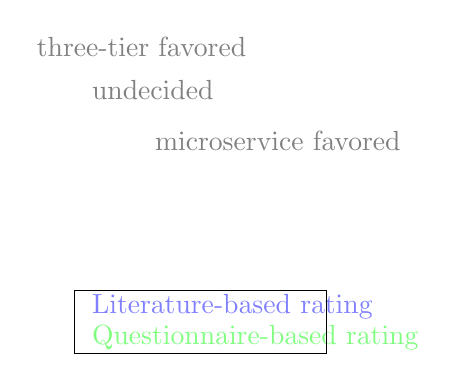
\begin{tikzpicture}
\tkzKiviatDiagram[scale=1.7,label space= 1.3, label distance=.1cm,
        radial  = 9,
        gap     = 1,  
        lattice = 3]{Resource efficiency with varying load, Horizontal scaling of components, Availability after component crash, Transaction consistency, Data consistency, Modifiability on \\ component level, Component reuse, Data segregation, Installability on premise}
\tkzKiviatLine[thick,color=blue,mark=none,
               fill=blue!20,opacity=.5](3,3,2,1,1,3,3,2,1)
\tkzKiviatLine[thick,color=darkgray,
               fill=green!20,opacity=.5](2.7,2.65,2.5,1.35,1.5,2.85,2.2,2.15,1.45) 
%\tkzKiviatLine[ultra thick,mark=ball,
%                 mark size=4pt,color =red](2,3.75,1,1.5,2)    
%\tkzKiviatGrad[prefix=,unity=1,suffix=](1)  
\node[color=gray, right] at (0.8,-0.7) {three-tier favored};
\node[color=gray, right] at (1.5,-1.25) {undecided};
\node[color=gray, right] at (2.3,-1.9) {microservice favored};
%legend
\node[color=blue!50, right] at (1.5,-4) {Literature-based rating};
\node[color=green!50, right] at (1.5,-4.4) {Questionnaire-based
 rating};
\draw (1.4, -3.8) -- (4.6, -3.8) -- (4.6, -4.6) -- (1.4, -4.6) -- (1.4, -3.8);
% Arrow
%\node (A) at (1.7, -5)[fill=black, draw,shape=circle, minimum size=0.2cm,inner sep=0]{};
%\node (B) at (4.3, -5)[]{};
%\draw [->] (A) edge (B);
%\node (C) at  (2.4, -5.2){};
%\node (D) at  (2.4, -4.8){};
%\draw [-] (C) edge (D)[color=gray];
%\node (E) at  (3.2, -5.2){};
%\node (F) at  (3.2, -4.8){};
%\draw [-] (E) edge (F)[color=gray]; 
%\node (G) at  (3.9, -5.2){};
%\node (H) at  (3.9, -4.8){};
%\draw [-] (G) edge (H)[color=gray]; 
\end{tikzpicture}
 \caption[KivatDiagram showing a graphical representation between literature and interview based evaluation regarding microservices and given quality scenarios]{Diagram showing a graphical representation of the results of literature based rating(blue) and interview based rating(green) regarding the question "How well are microservices suited to achieve the given quality scenario in comparison to a three-tier architecture". In total nine quality scenarios were evaluated. The graphic visualizes strong overlapping in the results between the two rating methods.}
\label{fig:kiviatQuality}
\end{figure}

A tabular representation of the data is listed in table \ref{res:table}.
The table shows literature and questionnaire-based rating.
All ratings are placed on a continuum between minus one and plus one.
It shows the relative rating for each scenario between microservices and three-tier architecture.
Again this refers to the question: Which architectural style is more suitable to achieve the given quality scenario.
Minus one stands for three-tier architecture favored, zero means undecided and plus one stands for microservice favored.

The difference column shows that the biggest outliers in rating show a difference of 0.8 and 0.5.
The outliers are going to be discussed in Section~\ref{res:discussion}.
The general tendency is that both methods produced strongly similar results.

\begin{table}[h]
  \renewcommand{\arraystretch}{1.2}
  \centering
  \sffamily
  \begin{footnotesize}
    \begin{tabular}{l l l l}
    \toprule
    \textbf{Quality attribute scenario} & \textbf{Literature-based rating} & \textbf{Questionnaire rating} & \textbf{Difference}\\
    \midrule
    Resource efficiency with varying load	&	1.0 	& 0.7 & 0.3\\
    Horizontal scaling of components	&	1.0		&	0.65  & 0.35\\
    Availability after component crash	&	0.0	&	0.5  & \textbf{0.5}\\
    Transaction consistency	&	-1.0		&	-0.65  & 0.35 \\
    Data consistency	&	-1.0		&	-0.5  & \textbf{0.5} \\
    Modifiability on component level	&	~1.0		&	0.85  & 0.15 \\    
    Component reuse	&	1.0		&	0.2  & \textbf{0.8} \\    
    Data segregation	&	0.0		&	0.15  & 0.15 \\    
    Installability on premise	&	-1.0		&	-0.55  & 0.45 \\                
    \bottomrule
    \end{tabular}
  \end{footnotesize}
  \rmfamily
  \caption[Quantified comparison between the literature and questionnaire-based evaluation.]{Quantified comparison between the literature and questionnaire-based evaluation. Negative one stands for three-tier architecture favored, zero means undecided and plus one stands for microservice favored. Differences larger or equal 0.5 in rating are highlighted in bold.}
  \label{res:table}
\end{table}


In conclusion, the results suggest that the evaluation of quality attribute scenarios done in Chapter~\ref{qua:qualitiesRating} based on literature research is backed up by the results of the questionnaire realized with microservice experts at SAP.

\clearpage

\subsection{Organizational qualities}

Four organizational requirements were evaluated by using literature-based research (see Section~\ref{quaMicro:tradeoffOrgRequirements}) and by using a questionnaire in regard to the question: ``Which architectural style (microservices or three-tier architecture) works better together with a given organizational requirement''.

Figure~\ref{fig:kiviatOrganizational} visualizes the results.
It shows the rating based on literature (blue) and the rating based on the questionnaire (green).
When looking at the overlapping of both quadrangles it becomes clear that both ratings share the same tendency regarding all four organizational requirements.

In detail the ratings show that:
\textit{Technical teams} and \textit{quality gates} strongly favor a three-tier architecture.
\textit{Explicit Interfaces} lightly and \textit{high development velocity} strongly favors microservices.
This is backed up by both literature as well as questionnaire based rating.

\begin{figure}
\centering
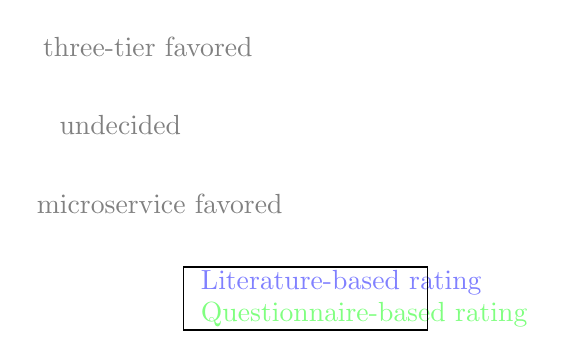
\begin{tikzpicture}
\tkzKiviatDiagram[scale=1.7,label space= 1.3, label distance=.1cm,
        radial  = 4,
        gap     = 1,  
        lattice = 3]{Technical teams, Explicit Interfaces, High development velocity, Quality gates}
\tkzKiviatLine[thick,color=blue,mark=none,
               fill=blue!20,opacity=.5](1,3,3,1)
\tkzKiviatLine[thick,color=darkgray,
               fill=green!20,opacity=.5](1.45,2.45,2.7, 1.55) 
\node[color=gray] at (0.95,-1) {three-tier favored};
\node[color=gray] at (0.6,-2) {undecided};
\node[color=gray] at (1.1,-3) {microservice favored};
%legend
\node[color=blue!50, right] at (1.5,-4) {Literature-based rating};
\node[color=green!50, right] at (1.5,-4.4) {Questionnaire-based rating};
\draw (1.4, -3.8) -- (4.5, -3.8) -- (4.5, -4.6) -- (1.4, -4.6) -- (1.4, -3.8);
\end{tikzpicture}
 \caption[KivatDiagram showing a graphical representation between literature and interview based evaluation regarding microservices and organizational requirements]{The diagram shows a graphical representation of the results of literature based rating(blue) and questionnaire based rating(green) regarding the question: "rate which architectural style (microservices and three-tier architecture) works better together with the given organizational requirement''. In total 4 organizational requirements were evaluated. The graphic again shows strong overlapping in the ratings between the two rating methods.}
\label{fig:kiviatOrganizational}
\end{figure}

\clearpage
\section{Discussion}
\label{res:discussion}
This section summarizes the interpretation of the results from the questionnaire.
The learnings reach beyond the pure numerical results.

\paragraph{Questionnaire results support literature-based evaluation}
The results of the questionnaire support the rating of the literature-based trade-off discussion from Chapter~\ref{qua:qualitiesRating}.
There were some outliers, like the scenarios \textit{component reuse}, \textit{data consistency} and \textit{availability after component crash}.
But even these are within a small margin and show the same tendency overall.

The biggest outliers were produced from the scenarios where the questionnaire participants engaged in conversation after the questionnaire. 
These scenarios left room for interpretation and different participants understood the scenarios differently.
This variance is partly reflected in the rating of these scenarios.
Especially regarding the \hyperref[quaMicro:s17]{scenario 17 - component reuse} participants were unsure about the type of component to be reused. 
The outliers are a pointer to the scenarios that might be formulated too vaguely and left room for interpretation. 

\paragraph{Application scenario rating failed}
Originally, the questionnaire was designed to match application scenarios with quality attributes.
The goal was do give a definitive guideline in which of the application scenarios to use microservices through an indirect mapping over quality attribute scenarios.
As elaborated in \ref{que:evalProcess} this approach failed.
This thesis suggests that the approach to match architectural styles with abstract application scenarios by rating quality attributes was flawed:

Firstly, if application scenarios are formulated in a rather general matter then it is hard to rate quality attributes for them at all. 
Different participants interpret the scenarios differently, which leads to unreliable results.

Secondly, company policies, team knowledge and other surrounding factors influence the decision for or against microservices strongly.
Therefore, it is hard to give a general advice with generally formulated application quality scenarios.
Even popular software architecture books, like \citep{Bass2012} do not recommend architectural styles for certain application types. 
The real world is just more complex than what an abstracted evaluation can conceive.

\paragraph{Researching the obvious}
In the questionnaire the participants were asked to rate 9 architectural qualities and 4 organizational requirements with regard to how well they fit together with microservices.
The presented architectural and organizational qualities mostly relate to the obvious and popularized qualities and disadvantages of microservices.
Supposedly without surprise, the results of the questionnaire support the evaluation done in the literature-based evaluation.

Did the questionnaire surface something unexpected? Probably, not.
Does this mean the questionnaire had no merit to it? No, it definitely had merit and that on different levels:

First of all, while it was probable, it was by no means certain that the questionnaires results will support the literature based evaluation.
In the end supporting arguments with different, unrelated sources makes them stronger.
This especially applies to a new concept like microservices, where the literature might not be as settled and approved as in other fields.
 
 %TODO small sample size could also explain
Secondly, while the answers in the questionnaire in general supported the evaluation there still were some interesting differences.
For example, regarding the component reuse scenario \hyperref[quaMicro:s17]{17} the standard deviation was 0.55, which is the highest value of derivation in the sample. 
That means that the amount of spread or distance from the mean is 0.55 when values between zero and two could be selected.
It seems that this topic is heavily discussed and the practitioners mostly disagree with each other whether microservices are better reusable than components in a three-tier architecture. 
This is an interesting observation as also literature writes very sparely on the reuse of microservices.

Thirdly and most importantly, the sophisticated discussion with participants about the questionnaire surfaced a general problem of this kind of architectural evaluation:
\begin{itemize}
\item Architectural trade-offs in real projects are much more complex than broad, general quality scenarios are able to express. Quality attribute scenarios seem to mainly have value if they are connected to a concrete use case.
\item The decision for an architectural style is dependent on much more than just quality attributes of the application. Factors like team knowledge, company organization and project size influence the architectural decisions heavily.
\end{itemize}

In conclusion a general architectural decision guidance cannot be provided purely on the basis of quality scenarios.
Every use case is different and though must be discussed individually.
The trade-off discussion in Chapter~\ref{qua:qualitiesRating} is a discussion starter for that.